

\clearpage
\subsection{The Byzantine merchant}
\label{sec:appendix:moj:byzantine}

Byzantium was an ancient city in modern-day Turkey, now called Istanbul. In 988 the Varangian Guard was formed by Emperor Basil II. This gave many Viking warriors the opportunity to join an elite guard for the Byzantine Emperor. Harald Hardrada was a great leader of the Varyags, as they were known.

\begin{display}{The byzantine stall}
	\label{fig:appendix:moj:places:byzantine:stall}
	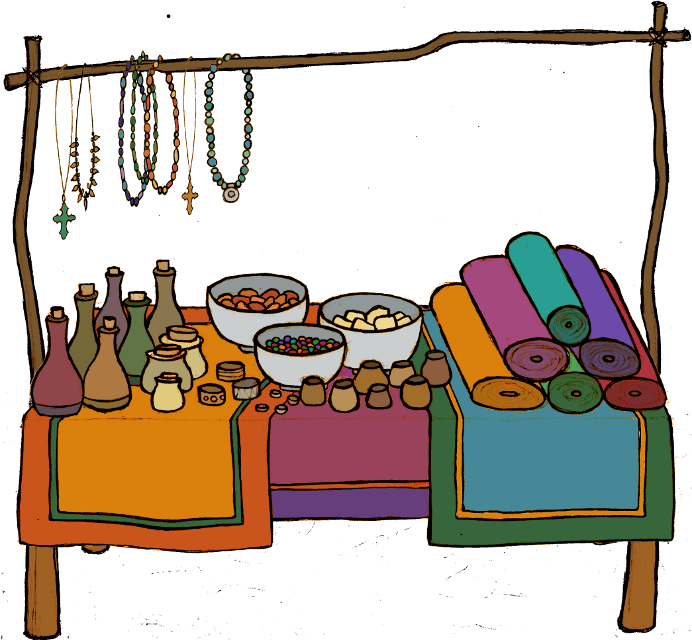
\includegraphics[width=0.65\columnwidth]{img/Jorvik/places/byzantine stall}
\end{display}

\begin{display}{The byzantine stall with a background and a merchant}
	\label{fig:appendix:moj:places:byzantine}
	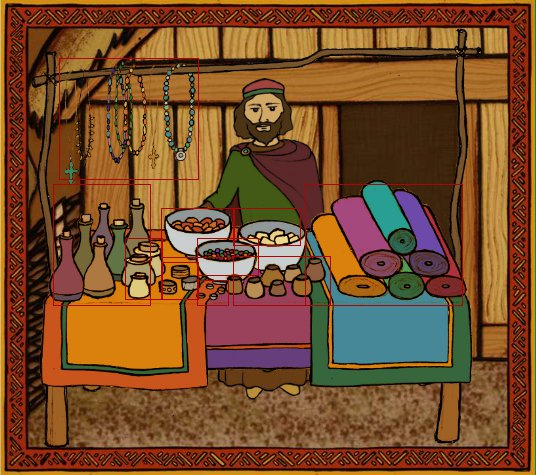
\includegraphics[width=0.65\columnwidth]{img/Jorvik/places/byzantine}
\end{display}
\clearpage


\begin{table}[ht!]
	\centering
	\begin{tabular}{ p{3cm} c }\toprule
		\textbf{Name:} & \multirow{5}{*}{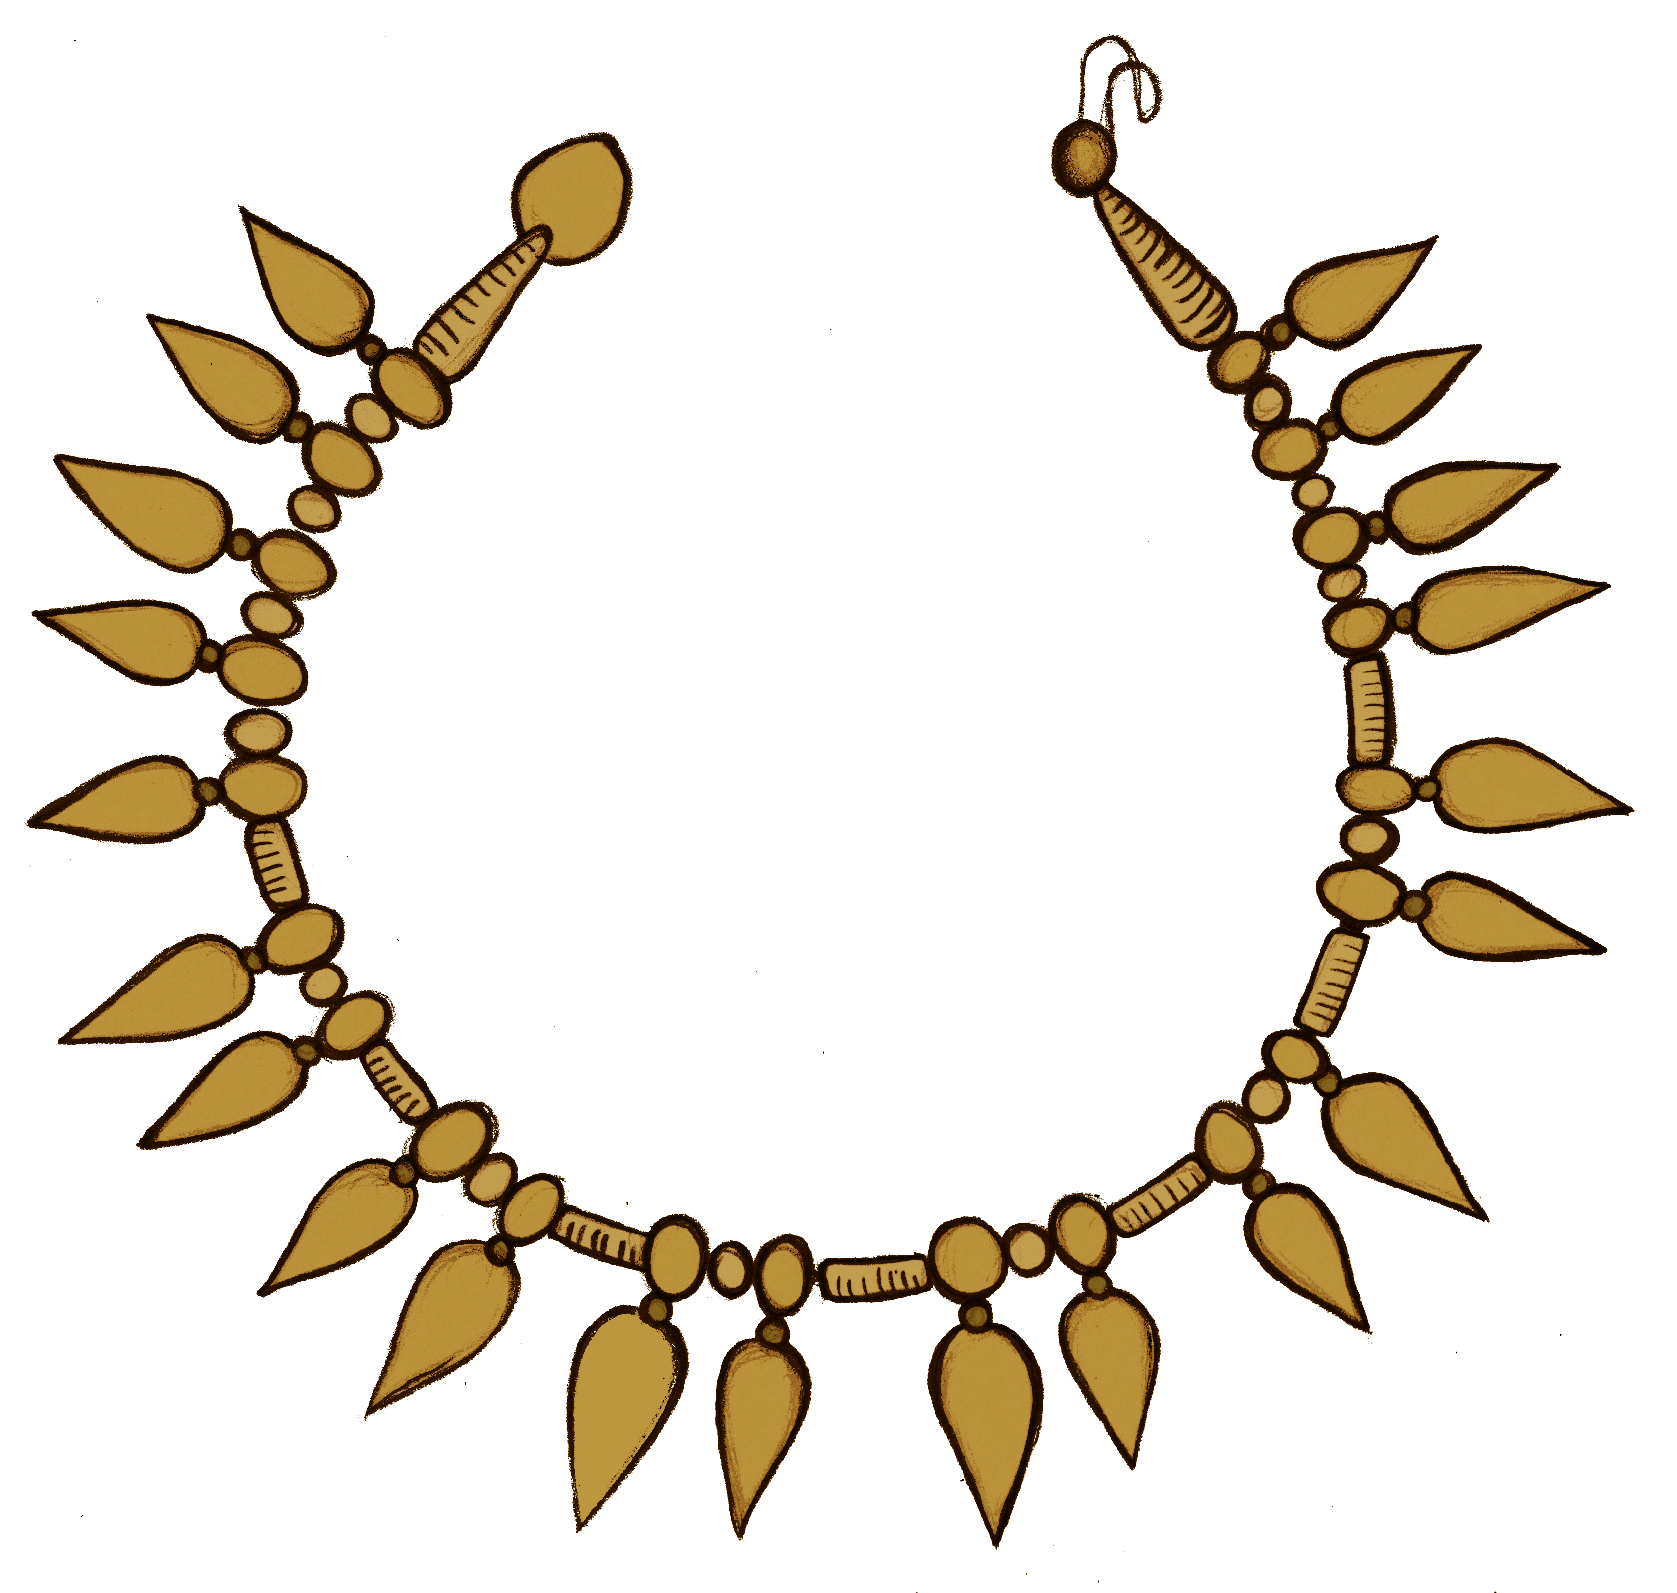
\includegraphics[height=30mm]{img/Jorvik/objects/byzantine/necklace}}\\
		Necklace & \\ 
		\textbf{Price:} & \\
		13.23 silver & \\ 
		\textbf{Description:} & \\
		\multicolumn{2}{p{12cm}}{The Byzantine Empire had an abundance of wealth so most jewellery was made out of gold and precious stones.}\\
		\bottomrule
	\end{tabular}
\end{table}

\begin{table}[ht!]
	\centering
	\begin{tabular}{ p{3cm} c }\toprule
		\textbf{Name:} & \multirow{5}{*}{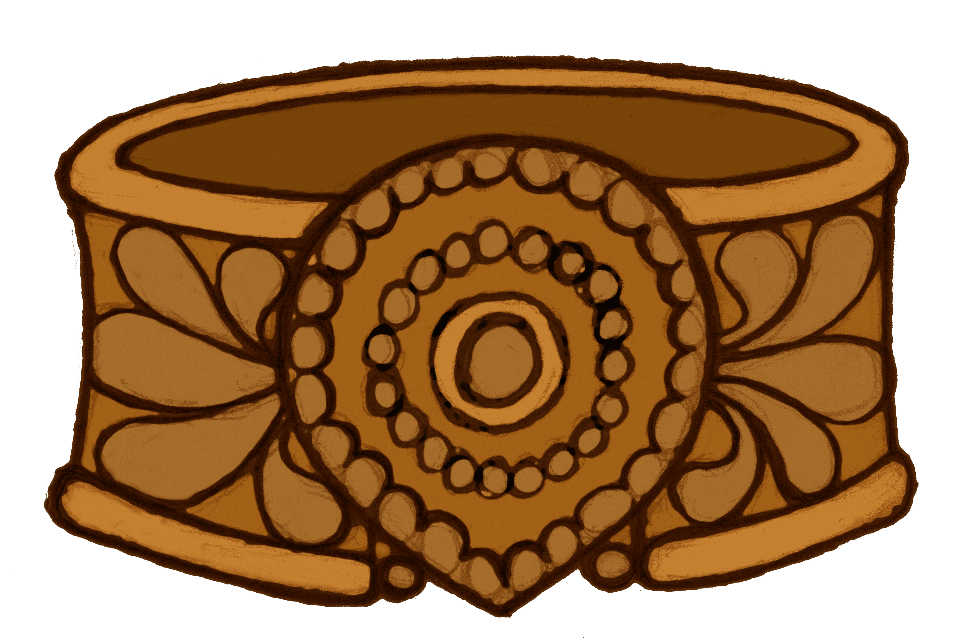
\includegraphics[height=30mm]{img/Jorvik/objects/byzantine/bracelet}}\\
		Bracelet & \\ 
		\textbf{Price:} & \\
		11.91 silver & \\ 
		\textbf{Description:} & \\
		\multicolumn{2}{p{12cm}}{Byzantine jewellery and art were influenced by religious symbols like the Christian cross. The patterns were very ornate and intricate.}\\
		\bottomrule
	\end{tabular}
\end{table}

\begin{table}[ht!]
	\centering
	\begin{tabular}{ p{3cm} c }\toprule
		\textbf{Name:} & \multirow{5}{*}{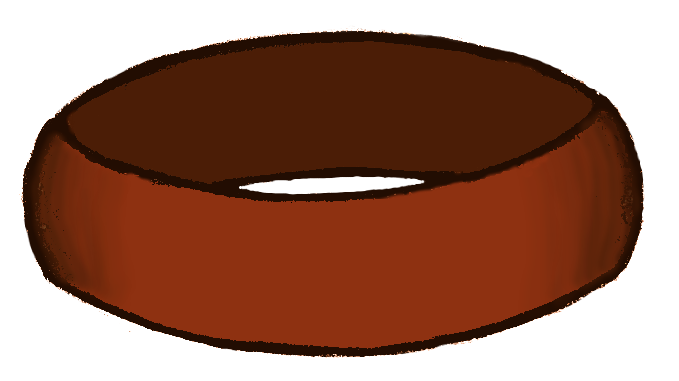
\includegraphics[height=30mm]{img/Jorvik/objects/byzantine/ring}}\\
		Ring & \\ 
		\textbf{Price:} & \\
		8.82 silver & \\ 
		\textbf{Description:} & \\
		\multicolumn{2}{p{12cm}}{The Byzantines used a lot of gemstones in their jewellery including beryl, garnets and pearls. They were popular all over the world and have been found in India and Persia (modern-day Iran).}\\
		\bottomrule
	\end{tabular}
\end{table}

\begin{table}[ht!]
	\centering
	\begin{tabular}{ p{3cm} c }\toprule
		\textbf{Name:} & \multirow{5}{*}{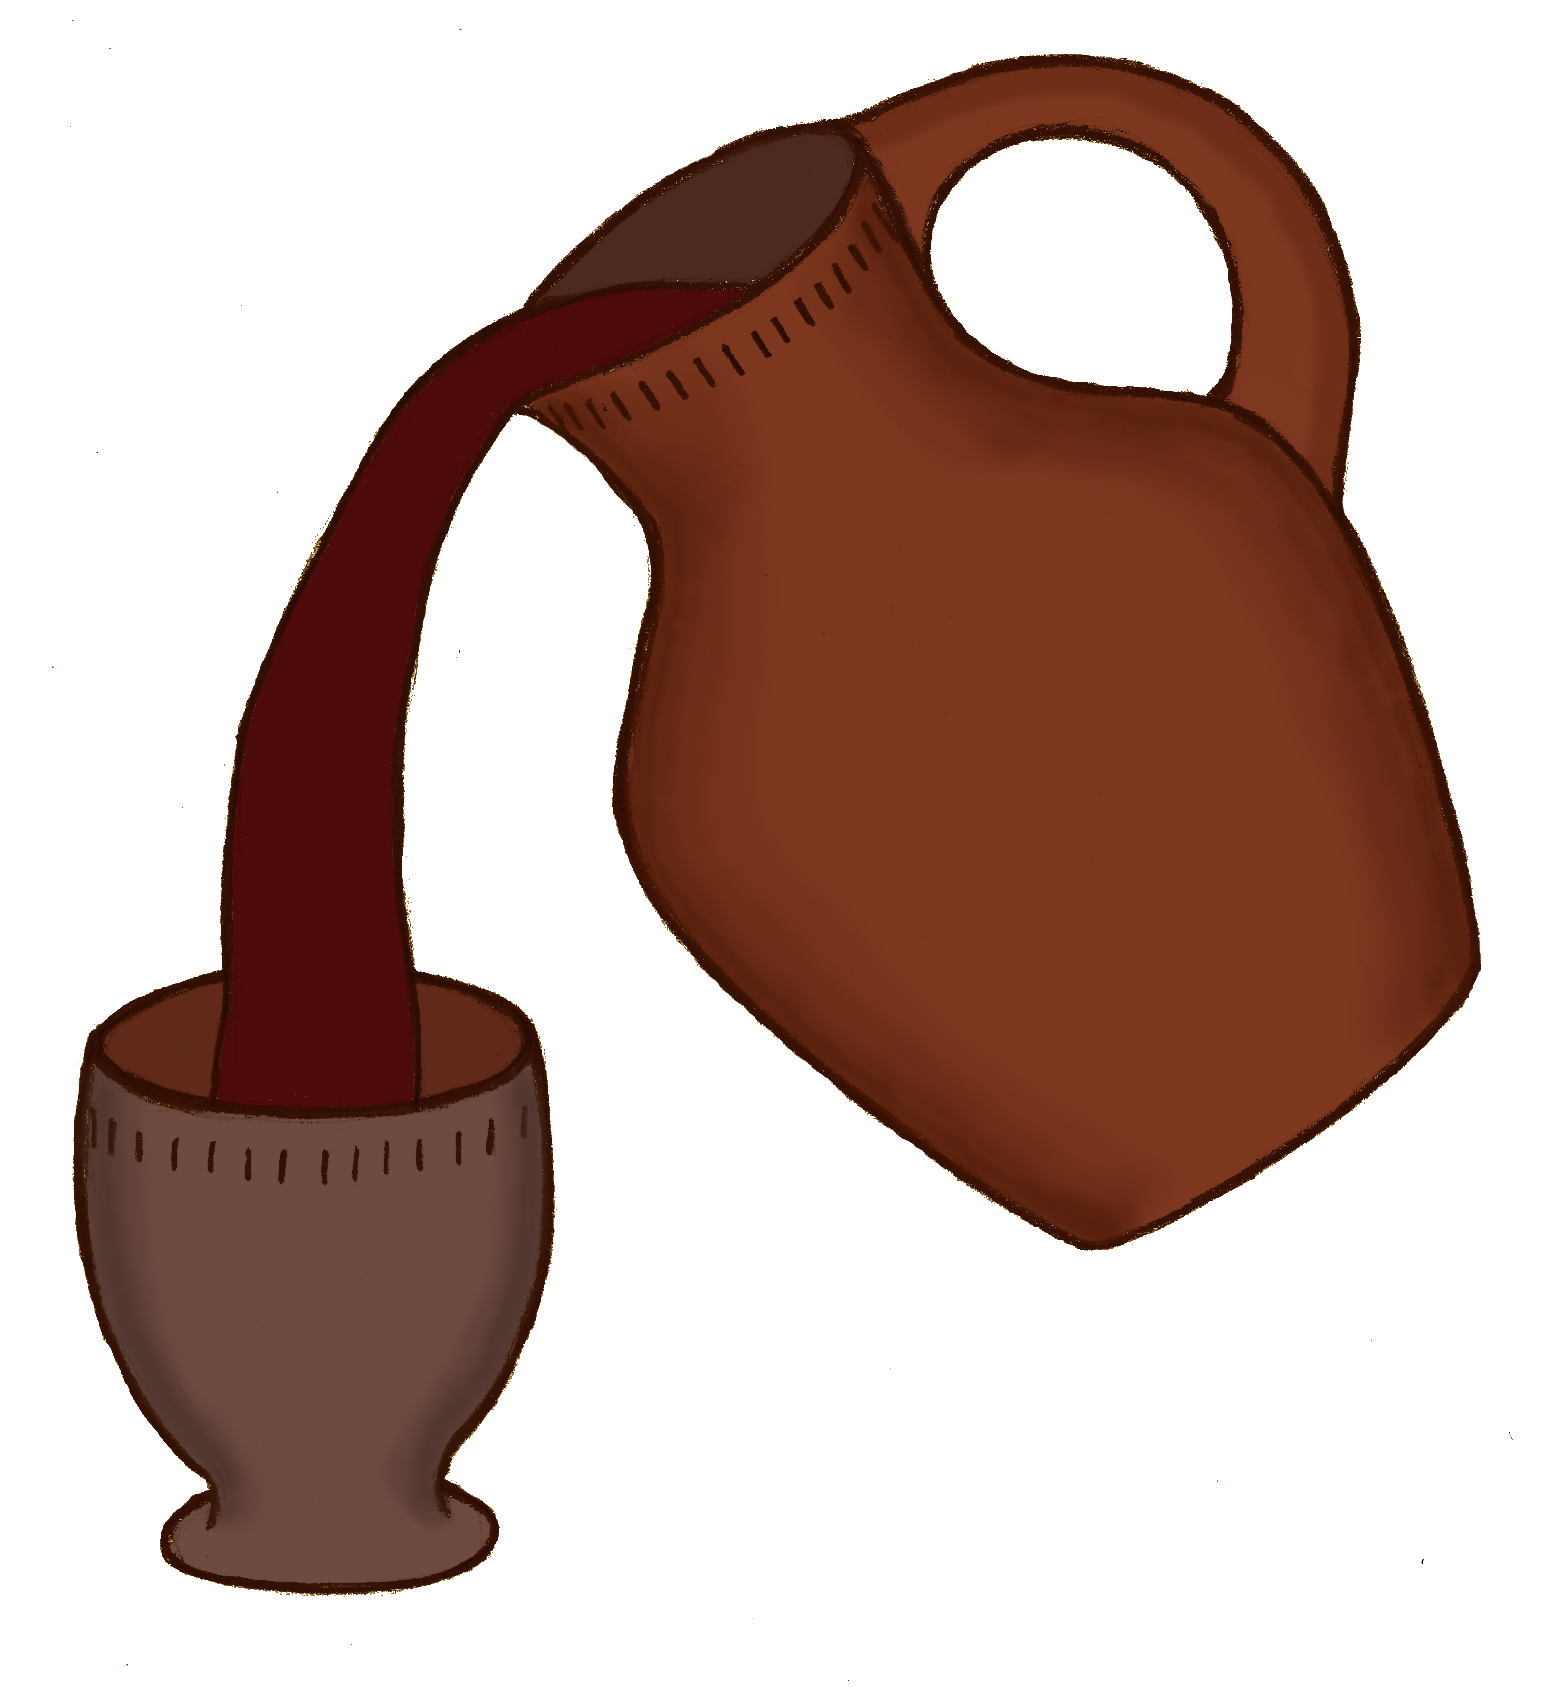
\includegraphics[height=30mm]{img/Jorvik/objects/byzantine/wine}}\\
		Wine & \\ 
		\textbf{Price:} & \\
		22.05 silver & \\ 
		\textbf{Description:} & \\
		\multicolumn{2}{p{12cm}}{Wine was imported from Byzantium and the kingdoms that now make up France and Germany, and was very expensive. Wine was a drink for the old and wise as the Norse God of Wisdom, Odin, only drinks mead or wine.}\\
		\bottomrule
	\end{tabular}
\end{table}

\begin{table}[ht!]
	\centering
	\begin{tabular}{ p{3cm} c }\toprule
		\textbf{Name:} & \multirow{5}{*}{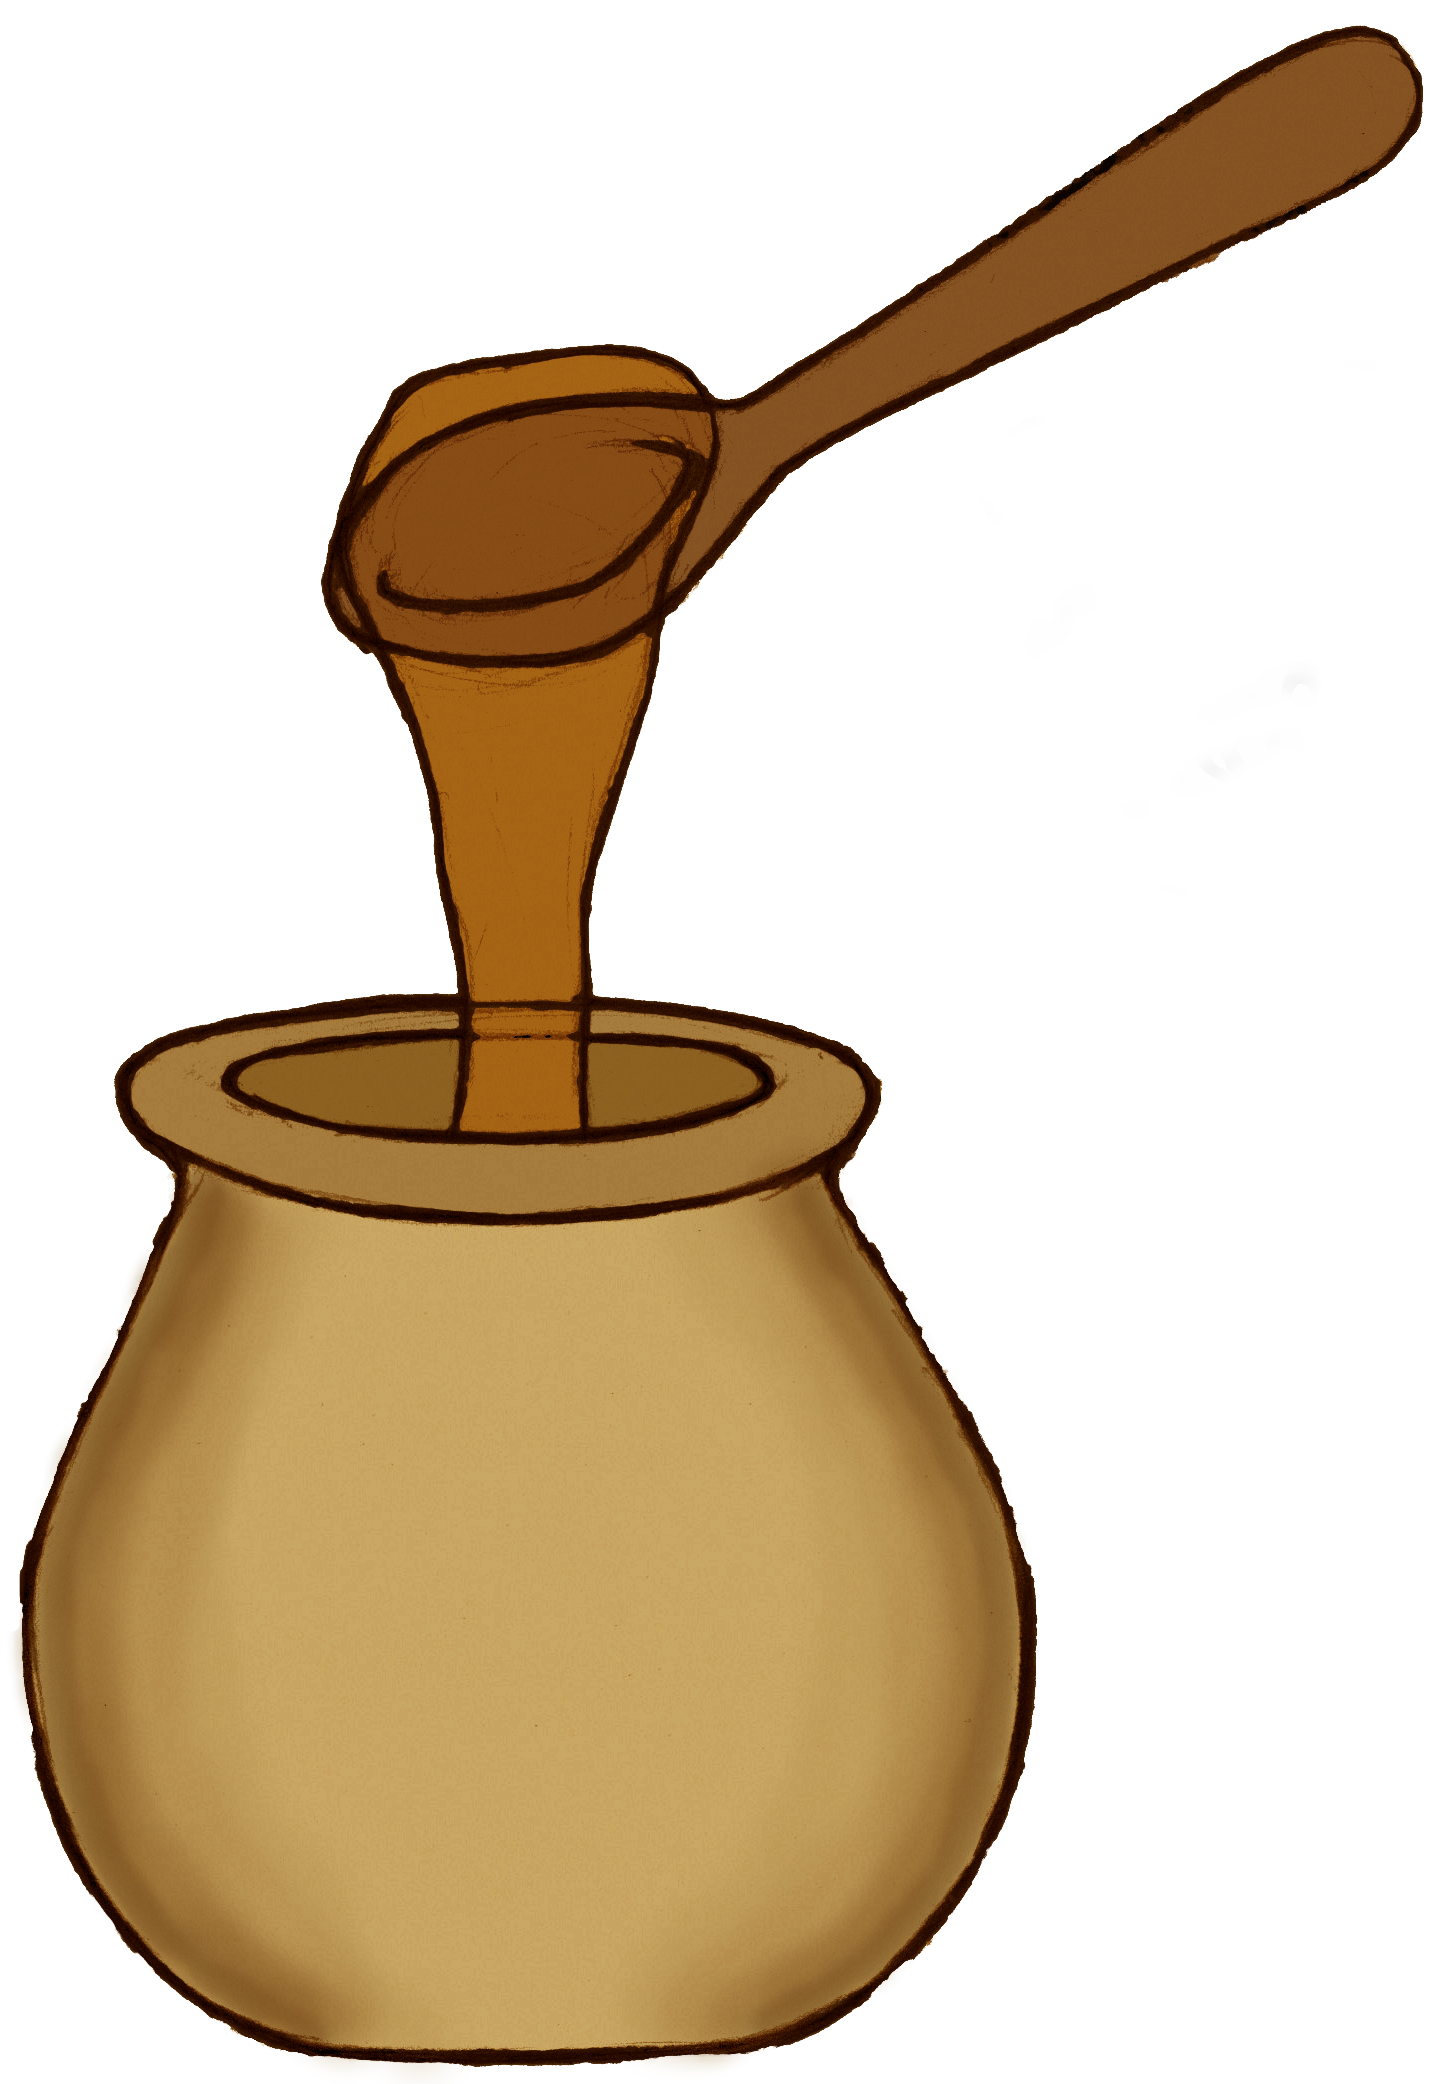
\includegraphics[height=30mm]{img/Jorvik/objects/byzantine/honey}}\\
		Honey & \\ 
		\textbf{Price:} & \\
		17.64 silver & \\ 
		\textbf{Description:} & \\
		\multicolumn{2}{p{12cm}}{Honey was a key ingredient in Viking mead often served at wedding feasts. Whilst there was local honey from other places in England, it was also imported from Russia.}\\
		\bottomrule
	\end{tabular}
\end{table}

\begin{table}[ht!]
	\centering
	\begin{tabular}{ p{3cm} c }\toprule
		\textbf{Name:} & \multirow{5}{*}{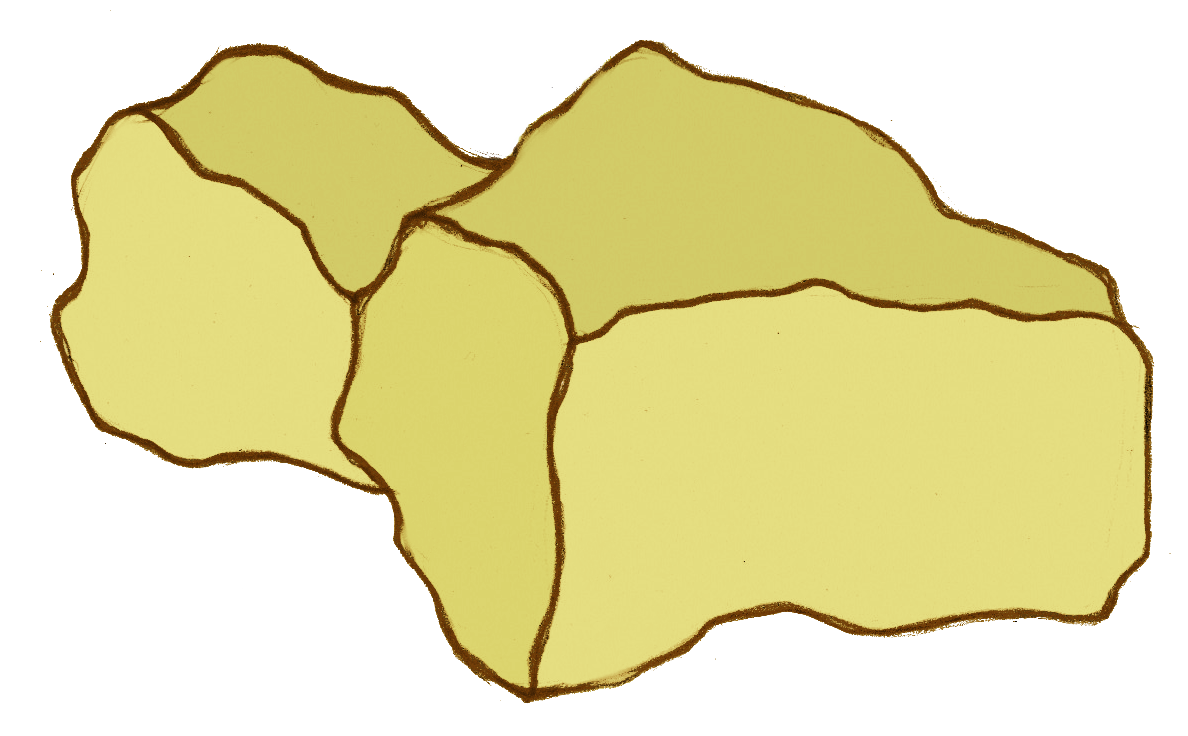
\includegraphics[height=30mm]{img/Jorvik/objects/byzantine/wax}}\\
		Wax & \\ 
		\textbf{Price:} & \\
		14.56 silver & \\ 
		\textbf{Description:} & \\
		\multicolumn{2}{p{12cm}}{Humanity has been using beeswax since civilisation began. Viking wood-turners used it to polish their products and leather-workers used it to seal the knots as they stitched the leather together using two needles.}\\
		\bottomrule
	\end{tabular}
\end{table}

\begin{table}[ht!]
	\centering
	\begin{tabular}{ p{3cm} c }\toprule
		\textbf{Name:} & \multirow{5}{*}{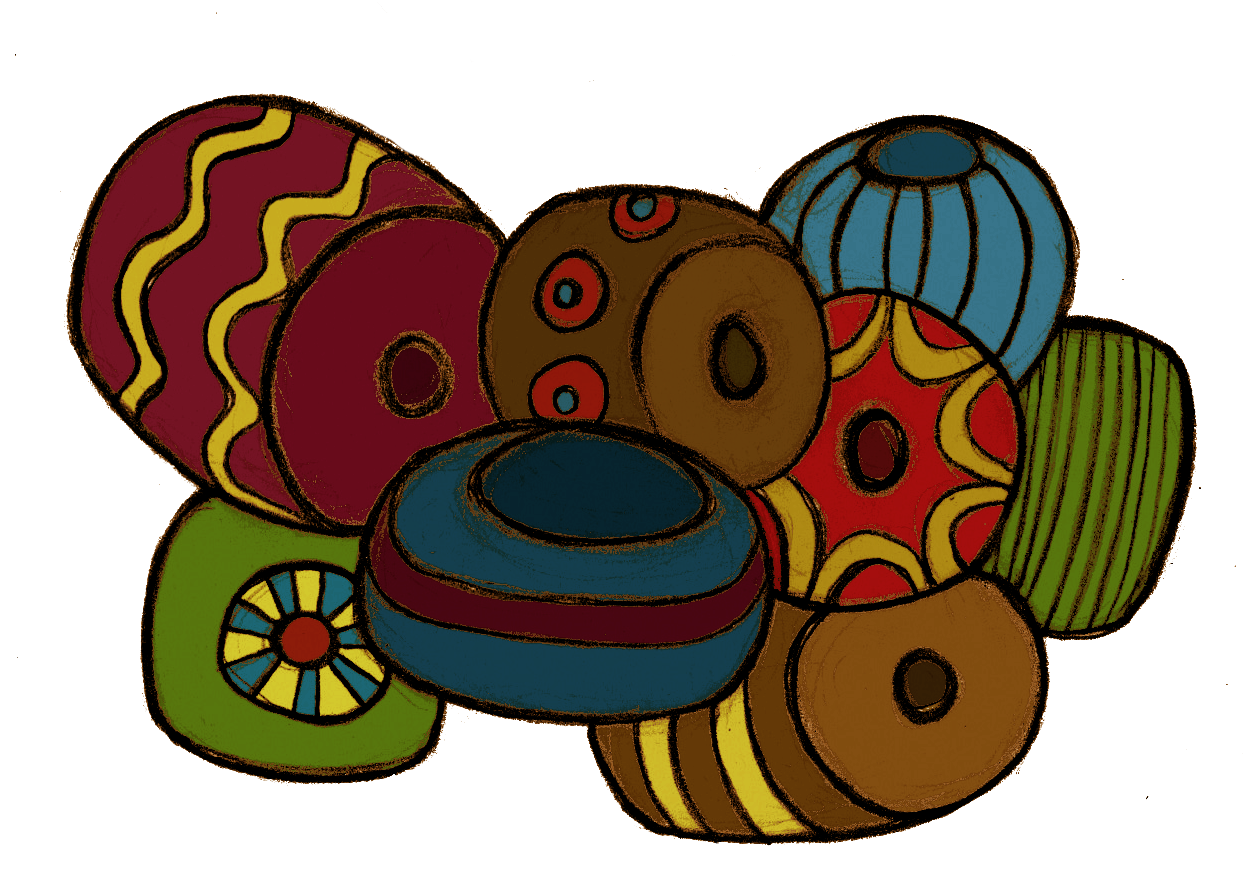
\includegraphics[height=30mm]{img/Jorvik/objects/byzantine/glass beads}}\\
		Glass Beads & \\ 
		\textbf{Price:} & \\
		1.59 silver & \\ 
		\textbf{Description:} & \\
		\multicolumn{2}{p{12cm}}{Glass workers could ornament the beads to make each one unique. They were worth a lot and were passed down to younger family members.}\\
		\bottomrule
	\end{tabular}
\end{table}

\begin{table}[ht!]
	\centering
	\begin{tabular}{ p{3cm} c }\toprule
		\textbf{Name:} & \multirow{5}{*}{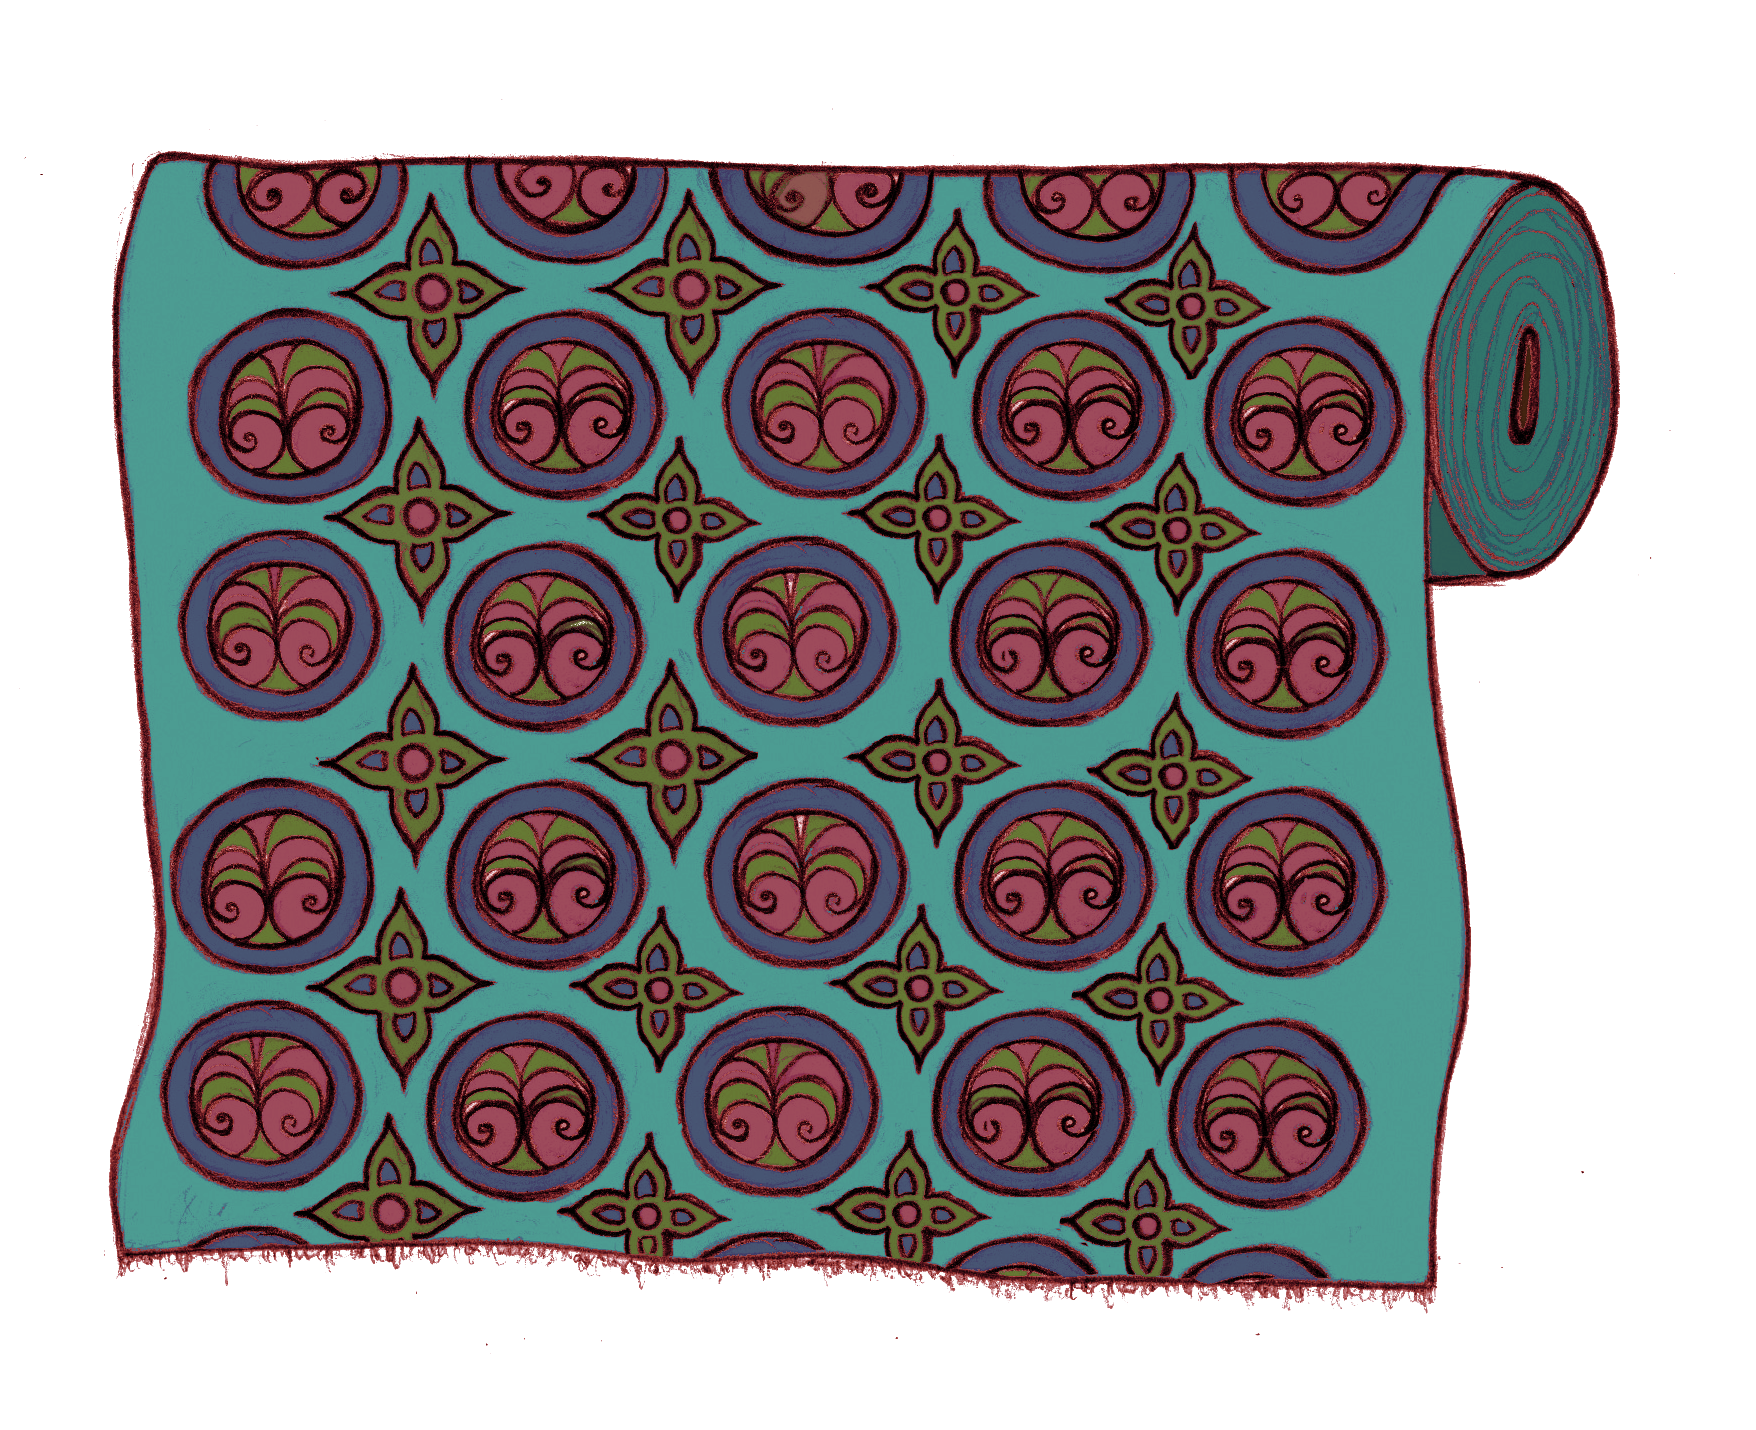
\includegraphics[height=30mm]{img/Jorvik/objects/byzantine/silk}}\\
		Silk & \\ 
		\textbf{Price:} & \\
		25.14 silver & \\ 
		\textbf{Description:} & \\
		\multicolumn{2}{p{12cm}}{Silk was a very expensive material and was worn by only the richest members of society. Lord Arinbjorn gave a custom-made silk robe as a Yule gift to his friend Egil Skallagrimson – this would have been very expensive!}\\
		\bottomrule
	\end{tabular}
\end{table}

\begin{table}[ht!]
	\centering
	\begin{tabular}{ p{3cm} c }\toprule
		\textbf{Name:} & \multirow{5}{*}{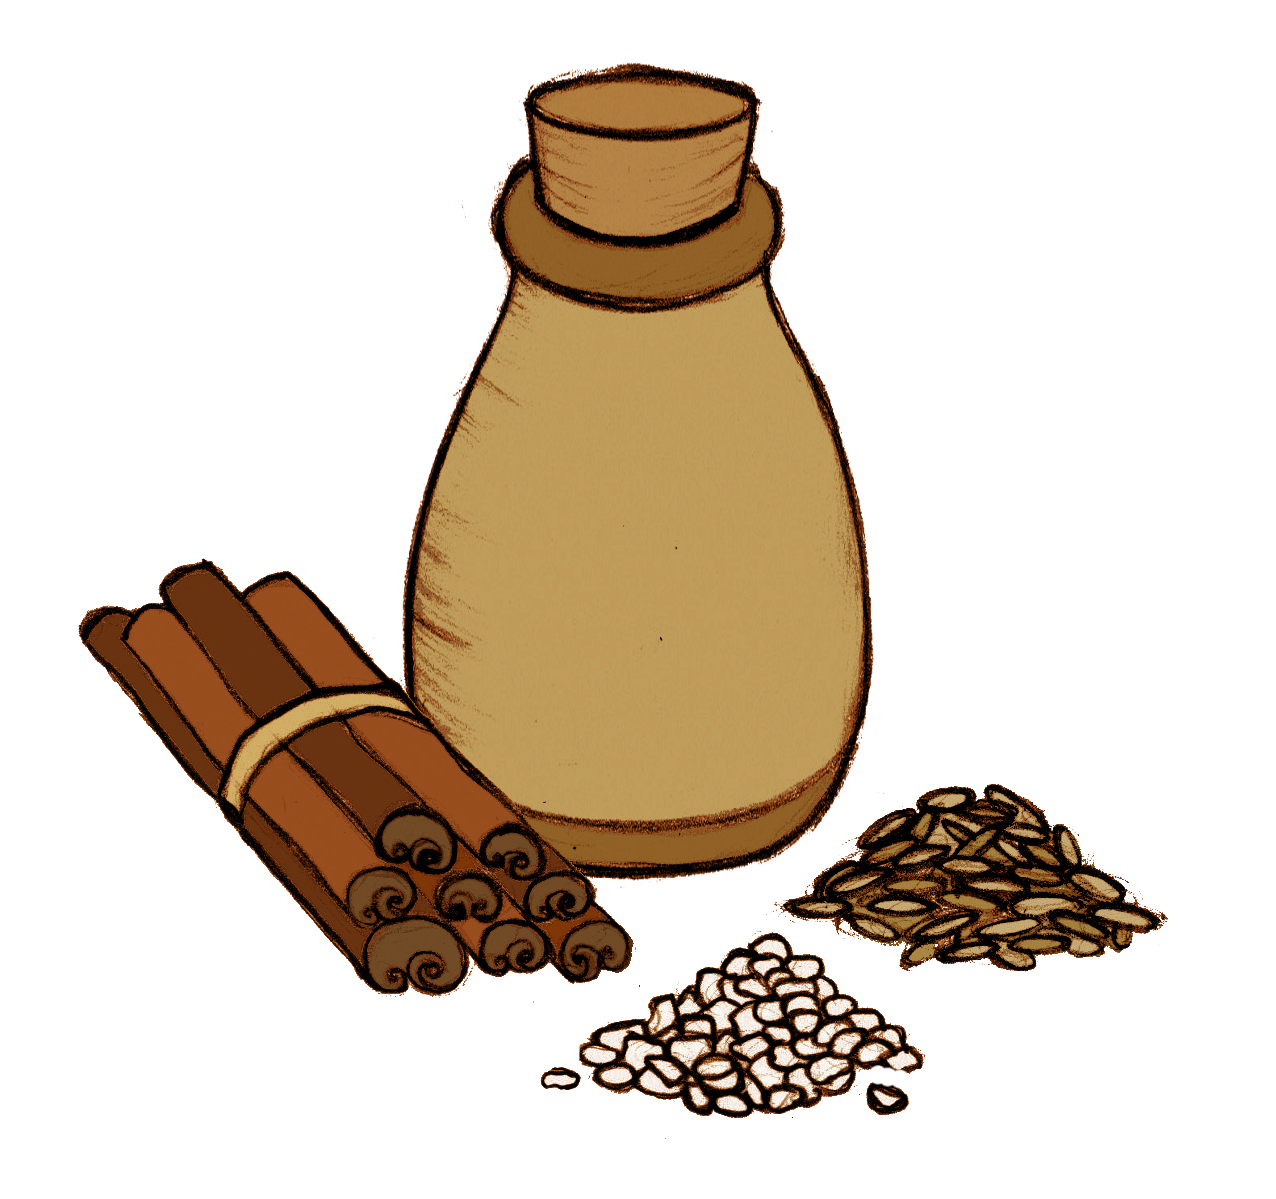
\includegraphics[height=30mm]{img/Jorvik/objects/byzantine/spice}}\\
		Spice & \\ 
		\textbf{Price:} & \\
		8.82 silver & \\ 
		\textbf{Description:} & \\
		\multicolumn{2}{p{12cm}}{Spices like coriander, cumin, mustard and saffron were imported and would have been expensive, but would have made for a very special wedding meal. }\\
		\bottomrule
	\end{tabular}
\end{table}

\begin{table}[ht!]
	\centering
	\begin{tabular}{ p{3cm} c }\toprule
		\textbf{Name:} & \multirow{5}{*}{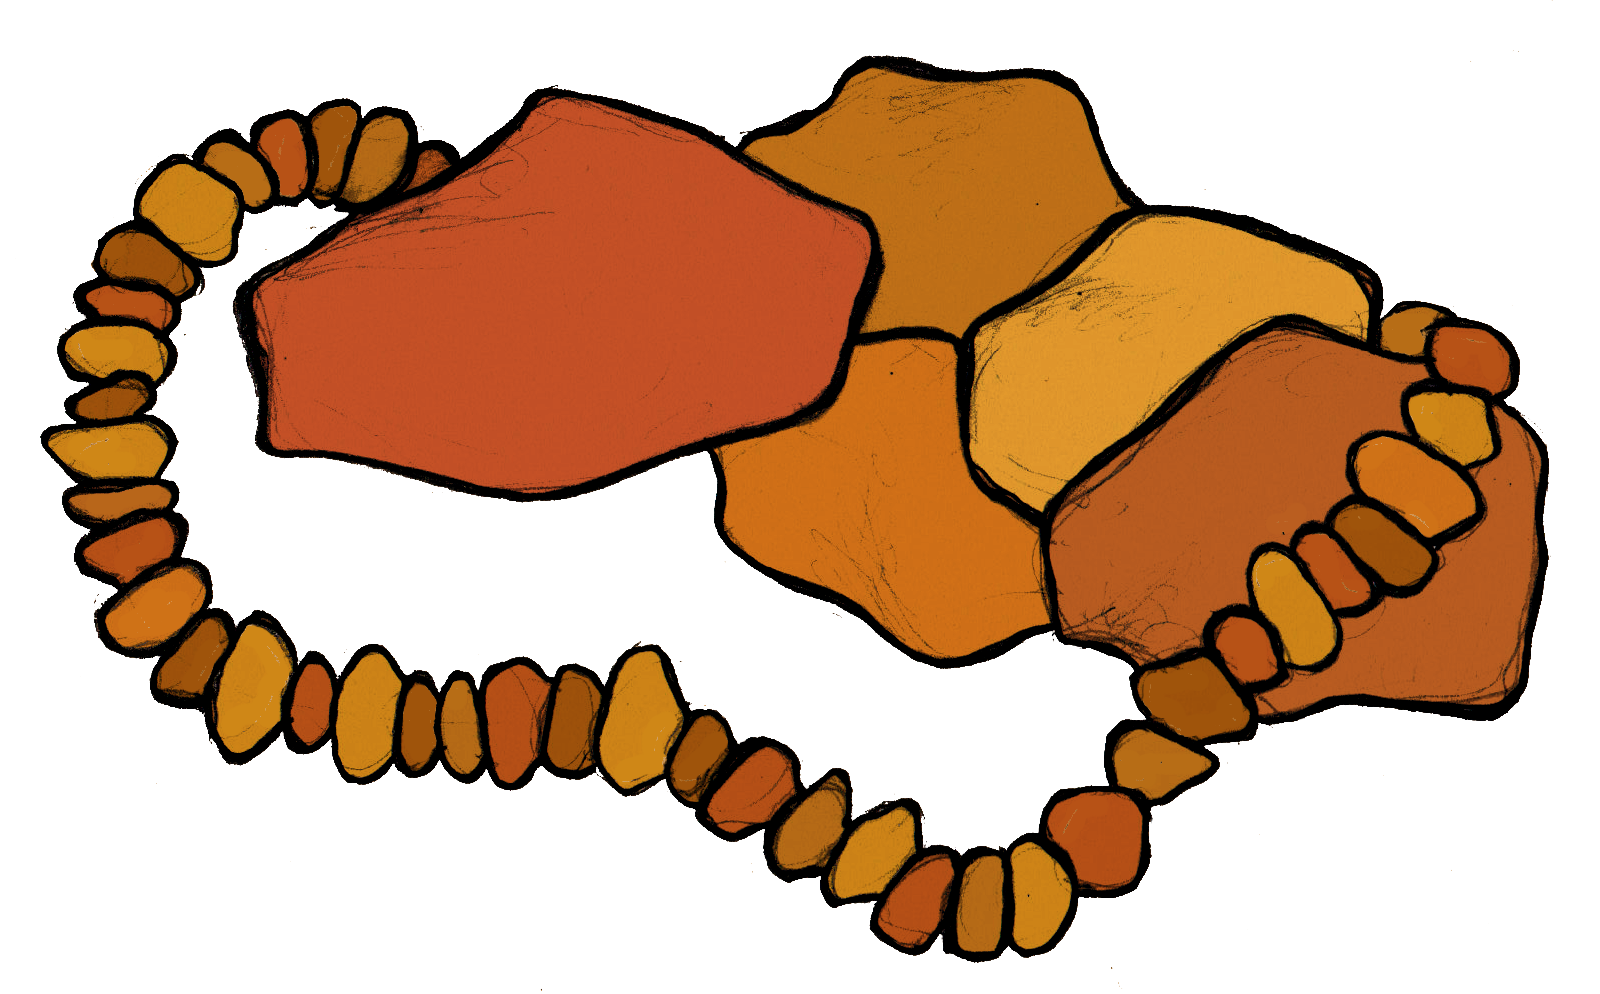
\includegraphics[height=30mm]{img/Jorvik/objects/byzantine/amber}}\\
		Amber & \\ 
		\textbf{Price:} & \\
		11.03 silver & \\ 
		\textbf{Description:} & \\
		\multicolumn{2}{p{12cm}}{Amber came from the Baltic regions and would have been traded both in jewellery and in its raw form. Amber was very expensive, it was believed that amber was the tears of the Norse goddess Freyja.}\\
		\bottomrule
	\end{tabular}
\end{table}